% !Mode:: "TeX:UTF-8"
\chapter{无人机辅助的双向车道边缘计算网络的鲁棒功率控制方法与轨迹优化}

\label{chap:table}
\section{引言}\label{section4-1}
\label{chap:introduction}
在前一个章节中,主要研究了车联网的地面通信网络,然而随着城市化建设的加深,道路网络越来越复杂,车辆的地面通信网络容易受到建筑物的遮挡,同时地面基站也难以覆盖越来越多的通信车辆。因此本章研究了作为前沿通信技术的无人机作为空中基站辅助车联网通信,并着重考虑了更加实际的双向车道的场景。无人机具有灵活与高机动性的特性,可以更好地解决如今越来越复杂的通信网络。由于本文考虑的车辆环境均为高速移动场景,固定轨迹的无人机难以适应实时变化网络拓扑环境,因此实时优化无人机的飞行的航迹有助于提高辅助车辆通信的服务质量。此外,无人机飞行与作为空中基站时均为耗能设备,所以整个系统的能量效率也应备受关注。

综上所述,本章研究了一个双向车道下无人机辅助车辆网络能效最大化的场景,在这个网络中,车辆高速行驶于双向的高速公路上,地面基站位于道路的一侧,随着对向行驶的车辆的高速移动,向右行驶的车辆会逐渐驶出当前通信小区,无法与地面基站进行通信,此时,无人机可作为空中基站以接收车辆通信信号。无人机以固定的高度平行于道路进行无障碍飞行,我们提出的算法可以实时的判断当前时隙车辆如何选择通信对象使得系统的能量效率最大化。本章的贡献可以做出如下总结:首先,本章提出了一种无人机辅助双向车道场景下规划无人机航迹的系统模型,为了提高整个网络系统的能量效率,我们采用丁克尔巴赫方法与定价机制使得系统在最小的能耗下可以最大化总吞吐量,为了保证地面车辆用户的服务质量,在优化问题中建立了时变的车辆移动模型下的概率约束,尽可能地描述信道的不确定性。
\section{系统模型}\label{section4-2}
本章考虑了一个天地一体化网络,其中车辆行驶于双向的高速公路上,无人机从基站附近起飞,缓存基站提供的资源供道路上的车辆下载,因为是双向车道,基站位于坐标原点,高度为$h_0$,路边单元RSU的位置为$dd$,$D_R$代表了路边单元的覆盖范围的半径长度,
我们规定向右为正方向,定义车道索引$L=1$为车辆向右行驶,$L=-1$为向左行驶,由于基站位置固定,随者时间的推移,不可避免地存在一个方向的车辆会远离基站,势必影响其通过基站获取信息,此时,无人机向着基站的右方飞去,进而帮助远离基站的车辆获取需要的信息。
为了决策道路上的车辆需要从无人机还是基站获取信息,我们根据由一阶马尔可夫过程预测到车辆到基站的信道状态信息与车辆与空中基站无人机视距链路得到的信道状态信息分别得出车辆与两个数据中中心通信的信噪比,车辆会选择信噪比较大的一方请求资源,$x_m\left[t\right]=1$为车辆选择无人机进行通信,反之车辆选择基站进行通信。

在时隙$t$内,无人机的水平坐标为$q_U\left[t\right]=\left\{x_u\left[t\right],y_u\left[t\right]\right\}$
无人机在距离路面高度为$H$进行无障碍飞行,其飞行最大速度为$V_{max}$,车辆$M$的初始水平位置为$q_M\left[0\right]=\left\{x_0,y_0\right\}$,
假设车辆以速度$\nu_m$匀速直线行驶,根据之前定义的车道索引可以得出车辆$M$在第$t$时刻的水
平位置变化为$x_m\left[t\right]=x_0+l\nu_m t$,车辆$M$的水平位置 $q_M=\left\{x_m\left[n\right],y_0\right\}$
根据位置信息我们可以得到在第$t$时刻的距离信息
车辆$M$在$t$时隙与路边单元的距离为${{d}_{m,R}}\left[ t \right]=\left\| {{q}_{M}}\left[ t \right]-{{q}_{R}} \right\|=\sqrt{{{x}_{m}}{{\left[ t \right]}^{2}}+{{y}_{0}}^{2}+{{H}^{2}}}$
,车辆$M$在$t$时隙与无人机的距离为
$
{{d}_{m,U}}\left[ t \right]=\left\| {{q}_{M}}\left[ t \right]-{{q}_{U}}\left[ t \right] \right\|=\sqrt{{{\left( {{x}_{m}}\left[ t \right]-{{x}_{u}}\left[ t \right] \right)}^{2}}+{{\left( {{y}_{m}}\left[ t \right]-{{y}_{u}}\left[ t \right] \right)}^{2}}+{{H}^{2}}}\
$.系统模型如图 \ref{systemuav}所示。
\begin{figure}[hptb!]
 \centering\small
 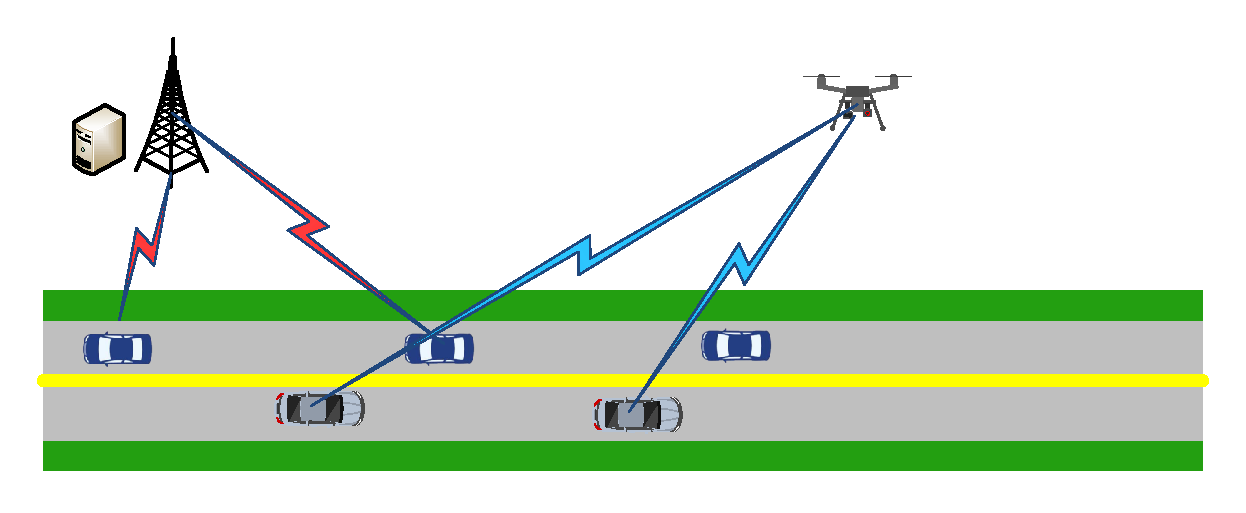
\includegraphics[width=0.6\textwidth]{systemuav}
 \Figcaption{无人机的系统模型}\label{systemuav}
\end{figure}

\subsection{车辆与地面基站通信计算与能耗模型}\label{section4-2-1}
由于车辆移动的快速性,对于车辆与路边单元的V2I通信,构建类似于前一章的一阶马尔可夫过程,在第$t$时刻的信道状态信息由前一时刻的状态预测得出,
即
\begin{equation} \label{E4-1}
%{\widetilde{g}}_{i,j}^k=L_{i,j}^2{\widetilde{h}}_{i,j}^2\xi_{i,j}^2
%h=\xi\tilde{h}+\sqrt{1-{{\xi }^{2}}}\zeta\    {\widetilde{g}}_{i,j}^k=L_{i,j}^2{\widetilde{h}}_{i,j}^2\xi_{i,j}^2
%{\widetilde{h}}_{m,R}=L_{m,R}^2{\widetilde{h}}_{m,R}^2\xi_{m,R}^2
h_{m}={\widetilde{h}}_{m}^2+{\hat{h}_{m}}^2,
\end{equation} \label{E4-2}
这里的${\widetilde{h}}_{m}$是一个观测值,${\hat{h}}_{m}$是一个服从参数为$a=\frac{1}{{L_{i,j}^k}^2({1-{\zeta_{i,j}^k}^2})}$的指数分布。
在第$t$个时隙,地面基站收到的第$m$辆车的信噪比(SNR)可以表示为:
\begin{equation}
\gamma_{m,R}\left[t\right]=\frac{p_m\left[t\right]h_{m,R}\left[t\right]}{\sigma^2}
\end{equation} \label{E4-3}
根据香农容量定理,车辆向地面基站的传输速率可以表示为:
\begin{equation}
R_{m,R}\left[t\right]=\log_2{\left(1+\gamma_{m,R}\left[t\right]\right)}
\end{equation}
车辆向地面基站传输的数据量可以表示为,
\begin{equation} \label{E4-4}
{{L}_{m,R}}={{B}_{0}}\underset{m=1}{\overset{M}{\mathop{\sum }}}\,\underset{t=1}{\overset{T}{\mathop{\sum }}}\,{{x}_{m}}\left[ t \right]R_{m,R}\left[t\right],
\end{equation}
其中$B_0$表示带宽,${{x}_{m}}\left[ t \right]=1$表示车辆当前时刻选择向地面基站传输数据,${{x}_{m}}\left[ t \right]=0$反之。


附属于路边单元的边缘服务器可以为收到的车辆数据进行数据计算处理
,因此计算卸载过程需要计算
资源,执行协作计算模型分裂的子任务。第$m$个车辆
的整个计算任务记为$A_m$,在某个时隙当其将任务分给路边单元时记为
$A_{R,m}={{z}_{m}}A_m$
我们定义$f_R$是路边单元的边缘服务器的CPU的加速频率,则计算时间可以表示为:
\begin{equation} \label{E4-4add}
t_{m}^{mec}=\frac{A_{R,m}}{f_R} \quad m \in \mathcal{M}.
\end{equation}
%同时我们使用瞬时的传输速率代替平均上传速率,由此可以得到车辆任务的上传时间为:、
%这里,我们将网络效用H(Am,i)定义为与访问子任务相关的卸载任务的计算满意度

车辆向地面基站路边单元通信时的传输能耗计算如下:
\begin{equation} \label{E4-5}
{{E}_{m,R}}=\underset{m=1}{\overset{M}{\mathop{\sum }}}\,\underset{t=1}{\overset{T}{\mathop{\sum }}}\,{{x}_{m}}\left[ t \right]{{p}_{m}}\left[ t \right]\
\end{equation}
\subsection{车辆与无人机通信与能耗模型}\label{section4-2-2}
对于车辆与无人机之间的通信中间没有障碍物遮挡,属于视距链路,构建了空中射频链路模型,
在第$t$个时隙,第$m$个车辆到无人机的信道增益为
\begin{equation} \label{E4-6}
h_{m,U}\left[t\right]=\frac{\varsigma_0}{{d_{m,U}\left[t\right]}^2}
\end{equation}
这里的$\varsigma_0$为单位距离1米下的功率增益,
%无人机与第$m$辆车之间的实时动态距离通过以下公式计算:
通过以上信息,无人机到车辆的传输速率为
\begin{equation} \label{E4-7}
R_{m,U}\left[t\right]=\log_2{\left(1+\gamma_{m,U}\left[t\right]\right)},
\end{equation}其中
\begin{equation} \label{E4-8}
\gamma_{m,U}\left[t\right]=\frac{p_m\left[t\right]h_{m,U}\left[t\right]}{\sigma^2},
\end{equation}表示车辆到无人机通信的信噪比,车辆向无人机空中基站传输的数据量可以表示为
\begin{equation} \label{E4-9}
%{{L}_{m,U}}={{B}_{0}}\underset{m=1}{\overset{M}{\mathop{\sum }}}\,\underset{t=1}{\overset{T}{\mathop{\sum }}}\,{{x}_{m}}\left[ t \right]{{\log }_{2}}\left( 1+{\gamma_{m,U}}\left[ t \right] \right)\
{{L}_{m,U}}={{B}_{0}}\underset{m=1}{\overset{M}{\mathop{\sum }}}\,\underset{t=1}{\overset{T}{\mathop{\sum }}}\,{{x}_{m}}R_{m,U}\left[t\right],
\end{equation}
其中$B_0$表示带宽,车辆向空中基站无人机通信时的传输能耗计算如下:
\begin{equation} \label{E4-10}
{{E}_{m,U}}=\underset{m=1}{\overset{M}{\mathop{\sum }}}\,\underset{t=1}{\overset{T}{\mathop{\sum }}}\,{{y}_{m}}\left[ t \right]{{p}_{m}}\left[ t \right]\
\end{equation}
由于无人机与路边单元之间具有良好的视距链路,因此我们认为车辆发送给无人机的数据
可以高效的传输到地面基站并由路边单元附属的边缘服务器进行数据处理。
\subsection{问题的定义}\label{section4-2-3}
在本节中,我们为无人机辅助的双向车道车辆制定了能效最大化问题。我们的目的是通过联合优化双向车道
上的车辆的发射功率以及无人机的轨迹来使得系统的总能效最大化.
首先,该网络通信系统的能效定义为
\begin{equation} \label{E4-11}
EE(\mathbf{P}, \mathbf{Q})=
{\frac{{{L}_{m}}\left( \mathbf{P}, \mathbf{Q} \right)}
{{{E}_{m}}\left( \mathbf{P} \right)}}
%EE(P,Q)=\sum\limits_{m=1}^{M}{\sum\limits_{n=1}^{N}{\frac{{{L}_{m,R}}\left[ n \right]+{{L}_{m,U}}\left[ n \right]}{{{E}_{m}}\left[ n \right]}}}
\end{equation}
式中的${{L}_{m}={L}_{m,R}+{L}_{m,U}}$是车辆向地面基站与空中基站发送的总的数据量,${E}_{m,R}$与${E}_{m,U}$分别是车辆与地面基站空中基站的能量消耗。
由于无人机飞行过程中会有能量的消耗,因此我们会更加关注车辆与无人机通信时的能耗问题,并考虑空中基站通信与地面基站通信的能量权衡,
因此系统的总功耗表示为${{E}_{m}=(1-\theta){L}_{m,R}+\theta{L}_{m,U}}$,其中$0\le \theta \le 1$是车辆与无人机通信时的能量成本的权重系数。
当$\theta$较大时意味着我们更加关注无人机的能耗成本。
最终的系统能效最大化问题如下表述:

\begin{align}
\max _{ \mathbf{P}, \mathbf{Q}, \mathbf{X} }  & EE(\mathbf{P}, \mathbf{Q}, \mathbf{X})                \label{E4-3end}\\
\text { s.t. }
& \Pr\left\{x_m\left[t\right]\gamma_{m,R}\left[t\right]+
y_m\left[t\right]\gamma_{m,U}\left[t\right]\geq \gamma_{th}\right\}\geq1-
\varepsilon_3, \forall m,t                                               \tag{\ref{E4-3end}{-1}}      \label{E4-3end1}\\  %信噪比中断概率约束
& 0\le p_m\left[t\right]\le p_{max}, \forall m                           \tag{\ref{E4-3end}{-2}}      \label{E4-3end2}\\  %功率阈值
& x_m\left[t\right] + y_m\left[t\right]=1, \forall m                     \tag{\ref{E4-3end}{-3}}      \label{E4-3end3}\\  %时隙分配加起来是一
& \frac{D_R}{\nu_m} \geq t_{m}^{mec}+t_{wired}                           \tag{\ref{E4-3end}{-4}}      \label{E4-3end4}\\  %这个是时隙的约束
& q_U^{n\mathrm{\ }+1}-q_U^{n\mathrm{\ }}\le tV_{max}, \forall m         \tag{\ref{E4-3end}{-5}}      \label{E4-3end5}    %无人机飞行轨迹
\end{align}

上式子中的\eqref{E4-3end1}表示了保证车辆通信的中断概率约束来保证服务质量,式子\eqref{E4-3end2}给出了
车辆最大最小发射功率的约束,式\eqref{E4-3end3}则代表了每个车辆每个时刻的任务只能向无人机或者地面基站
进行卸载,
 $\gamma_{th}$是信噪比的阈值为一个固定值,\eqref{E4-3end4}表示了需要调度车辆在其驶出路边单元覆盖范围
之前服务器要完成完成数据的计算,其中$t_{wired}$是路边单元向边缘服务器发送数据时的
固定时间。无人机的飞行轨迹受到\eqref{E4-3end5}的约束,


\section{能效最大化问题求解}\label{section4-3}
在本节中,上一章节的能效最大化问题会分解为两个子问题进行求解。对于难以求解的分式规划,可以使用丁克尔巴赫方法
将其转化为易于求解的减式规划进行求解。首先固定车辆的发射功率后求解无人机的飞行轨迹,然后固定无人机的飞行轨迹再求解
车辆的发射功率,如此进行交替迭代优化,直至算法收敛。注意到前一节中问题\eqref{E4-3end}是一个非凸的问题,我们提出了
一种联合功率分配与无人机轨迹规划的方案来有效地处理这个问题,
将问题\eqref{E4-3end}解耦成两个子问题。
\subsection{概率约束的近似与车辆发射功率优化问题}\label{section4-3-1}
在前一节的式\eqref{E4-3end1}中我们发现车辆的功率功率在概率约束中存在较为复杂的耦合关系,是难以直接求解的,
针对这种情况,我们将采用积分变换的方式将复杂的概率约束问题转化为较为简单的形式。

定理:对于\eqref{E4-3end1},车辆用户的中断概率约束
\begin{align}
\Pr\left\{x_m\left[t\right]\gamma_{m,R}\left[t\right]+y_m\left[t\right]\gamma_{m,U}\left[t\right] \geq \gamma_{th}\right\}\geq1-\varepsilon_3    \notag
\end{align}
等价于:
\begin{equation} \label{E4-13}
\begin{gathered}
p_m\left[t\right]x_m\left[t\right]\ln \left(1-a \varepsilon_3\right)+(\gamma_{th}-y_m\left[t\right]\gamma_{m,U})\left[t\right] a \sigma^2
\leq a p_m\left[t\right]x_m\left[t\right]\hat{h}_{m}\left[t\right]
\end{gathered}
\end{equation}
%\textcolor[RGB]{202,12,22}{巴拉巴拉}

证明:
\begin{align} \label{E4-14}
\frac{x_m\left[t\right]p_m\left[t\right]h_{m,R}\left[t\right]}{\sigma^2}\geq \gamma_{th}-y_m\left[t\right]\gamma_{m,U}\left[t\right] \\
\Leftrightarrow
p_m\left[t\right]{\widetilde{h}}_{m}\left[t\right]\geq \frac{{(\gamma_{th}-y_m\left[t\right]\gamma_{m,U}\left[t\right])\sigma^2}}{x_m\left[t\right]}
-p_m\left[t\right]{\hat{h}}_{m}\left[t\right]   \notag
\end{align}
%$\frac{{(SNR_{th}-y_m\left[t\right]\gamma_{m,U})\sigma^2}}{x_m\left[t\right]}$
因此车辆用户的中断概率约束做出重新表述如下:
\begin{align} \label{E4-15}
\Pr\left\{x_m\left[t\right]\gamma_{m,R}\left[t\right]+y_m\left[t\right]\gamma_{m,U}\left[t\right] \geq \gamma_{th}\right\}\geq1-\varepsilon_3    \\
\Leftrightarrow
\Pr\left\{{\widetilde{h}}_{m}\left[t\right]\geq \frac{{(\gamma_{th}-y_m\left[t\right]\gamma_{m,U}\left[t\right])\sigma^2}}{p_m\left[t\right]x_m\left[t\right]}
-{\hat{h}}_{m}\left[t\right]\right\}\geq1-\varepsilon_3                          \notag
\end{align}
由于随机变量$\widetilde{h}$的概率密度函数为$f_x={{e}^{-ax}}$,通过积分变换可得:
\begin{align} \label{E4-16}
&\int_{0}^{\frac{{(\gamma_{th}-y_m\left[t\right]\gamma_{m,U})\sigma^2}}{p_m\left[t\right]x_m\left[t\right]}
-{\hat{h}}_{m}\left[t\right]}{e^{-ax}dx}\le \varepsilon_3 \\
\Leftrightarrow
&p_m\left[t\right]x_m\left[t\right]\ln \left(1-a \varepsilon_3\right)+(\gamma_{th}-y_m\left[t\right]\gamma_{m,U}\left[t\right]) a \sigma^2
\leq a p_m\left[t\right]x_m\left[t\right]\hat{h}_{m}\left[t\right]   \notag
%GVRR.* P_m.*X' >= SNRth*Delta+ GVUU.*P_m.*Y'+log(1-e1)*P_m.*X'
\end{align}
为了表达方便,我们定义$\gamma_{m,U}\left[t\right]=p_m\left[t\right]\eta_{m,U}\left[t\right]$,其中$\eta_{m,U}\left[t\right]=h_{m,U}\left[t\right]/{\sigma^2}$,
将式子\eqref{E4-16}改写为:
\begin{equation} \label{E4-17}
p_m\left[t\right]x_m\left[t\right]\ln \left(1-a \varepsilon_3\right)+(\gamma_{th}-y_m\left[t\right]p_m\left[t\right]\eta_{m,U}\left[t\right]) a \sigma^2
\leq a p_m\left[t\right]x_m\left[t\right]\hat{h}_{m}\left[t\right]
\end{equation}

在求解车辆发射功率的过程中,需要每个时隙都要进行功
率分配与无人机轨迹规划并进行多次迭代,
关于车辆发射功率$p_m\left[t\right]$的子问题如下描述:
\begin{align}
\max _{ \mathbf{P}} &   ={\frac{{{L}_{m}}\left( \mathbf{P} \right)}
{(1-\theta){E}_{m,R}\left( \mathbf{P} \right)+\theta{E}_{m,R}\left( \mathbf{P} \right)}}         \label{E4-4end}\\
\text { s.t. }
& \eqref{E4-3end1},\eqref{E4-3end4}                                 \tag{\ref{E4-4end}{-1}}      \label{E4-4end1}
\end{align}
注意到问题\eqref{E4-4end}是一个分式规划问题,
为了将其转化为减式规划问题,拟采用丁克尔巴赫方法求解。
\begin{align} \notag
F(\chi)= & \max _{ \mathbf{P}} \sum_{t=1}^T \sum_{m=1}^M {B}_{0}x_{m}^{\left\{ l \right\}}\left[ t \right] %x_m\left[t\right]
\log_2{\left(1+p_m\left[t\right]\eta_{m,R}^{\left\{ l \right\}}\left[t\right]\right)}                         \\       \label{E4-5end}
& + \sum_{t=1}^T \sum_{m=1}^M {B}_{0}x_{m}^{\left\{ l \right\}}\left[ t \right]
\log_2{\left(1+p_m\left[t\right]\eta_{m,U}^{\left\{ l \right\}}\left[t\right]\right)}                         \\ \notag
& -\chi \sum_{t=1}^T \sum_{m=1}^M{(1-\theta)x_{m}^{\left\{ l \right\}}\left[ t \right]p_m\left[t\right]
+\theta y_{m}^{\left\{ l \right\}}\left[ t \right]p_m\left[t\right]}                                          \\ \notag
\text { s.t. }
& \eqref{E4-3end1},\eqref{E4-3end4}                                       \tag{\ref{E4-5end}{-1}}                      \label{E4-5end1}
\end{align}

上式中的$\eta_{m,R}^{\left\{ l \right\}}\left[t\right]=h_{m,R}\left[t\right]/{\sigma^2}$,
$\eta_{m,U}^{\left\{ l \right\}}\left[t\right]=h_{m,U}\left[t\right]/{\sigma^2}$
在每$l$次迭代时视为常数,对于凸问题\eqref{E4-5end},
我们可以构建拉格朗日函数并运用拉格朗日对偶法进行求解:
\begin{align}\label{E4-20}
&L\left(\mathbf{p},\lambda\right)\\
&=\sum_{t=1}^T \sum_{m=1}^M {B}_{0}x_{m}^{\left\{ l \right\}}\left[ t \right] %x_m\left[t\right]
\log_2{\left(1+p_m\left[t\right]\eta_{m,R}^{\left\{ l \right\}}\left[t\right]\right)}+                                                      \notag
\sum_{t=1}^T \sum_{m=1}^M {B}_{0}y_{m}^{\left\{ l \right\}}\left[ t \right]
\log_2{\left(1+p_m\left[t\right]\eta_{m,U}^{\left\{ l \right\}}\left[t\right]\right)}                     \\                                \notag
&-\chi \sum_{t=1}^T \sum_{m=1}^M{(1-\theta)x_{m}^{\left\{ l \right\}}\left[ t \right]p_m\left[t\right]
+\theta y_{m}^{\left\{ l \right\}}\left[ t \right]p_m\left[t\right]} \\
&-\sum\limits_{t=1}^{T}{\sum\limits_{m=1}^{M}{{{\lambda }_{m,t}}}}\left( ({{\gamma }_{th}}-{{y}_{m}}\left[ t \right]{{p}_{m}}\left[ t \right]{{\eta }_{m,U}}\left[ t \right])a{{\sigma }^{2}}-a{{p}_{m}}\left[ t \right]{{x}_{m}}\left[ t \right]{{{\hat{h}}}_{m}}\left[ t \right]+{{p}_{m}}\left[ t \right]{{x}_{m}}\left[ t \right]\ln \left( 1-a{{\varepsilon }_{3}} \right) \right)                                                                 \notag
%&-\sum_{t=1}^T\sum_{m=1}^M\lambda_{m,t}\Big[  (\gamma_{th}-y_m\left[t\right]p_m\left[t\right]\eta_{m,U}\left[t\right]) a \sigma^2 \\
%&-a p_m\left[t\right]x_m\left[t\right]\hat{h}_{m}\left[t\right]+ p_m\left[t\right]x_m\left[t\right]\ln \left(1-a \varepsilon_3\right)\Big]  \notag,
\end{align}
其中的拉格朗日乘子$\lambda_{m,t}\geq 0$,则\eqref{E4-20}的拉格朗日对偶函数表示为:
\begin{equation} \label{E4-21}
D(\mathbf{\lambda})=\max _{\substack{0 \leq P_m[t] \leq P_{\max }}} L\left(\mathbf{p_m},\mathbf{\lambda}\right)
\end{equation}
其中\eqref{E4-21}的对偶问题为:
\begin{equation} \label{E4-22}
\min_{\substack{\lambda_{m,t}\geq 0}} D\left(\mathbf{p_m},\mathbf{\lambda}\right)
\end{equation}
问题\eqref{E4-22}是一个凸问题且满足Karush-Kuhn-Tucker(KKT)条件,
在使用KKT条件的类似求解过程中可令其一阶导数为等于零:
\begin{align}\label{E22add}
\frac{\partial D\left(\mathbf{p_m},\lambda,\mu\right)}{\partial p_i}=A_i-\Bigl[\sum_{j=1,j\neq i}^{M}\left(A_j\frac{{\bar{\gamma}}_j\left(e^{\widetilde{p}}\right){\bar{G}}_{k,j}}{e^{{\widetilde{p}}_j}{\bar{G}}_{j,j}}\right)\\
+\lambda_i\mathrm{\Pi}_ie^{-{\widetilde{p}}_i}+\mu_i{\hat{g}}_{i,j}^k\Bigl]e^{{\widetilde{p}}_i}=0\notag,
\end{align}
\textcolor[RGB]{202,12,22}{再加点橙子梯度}
\subsection{无人机飞行轨迹规划问题}\label{section4-3-2}
%\textcolor[RGB]{202,12,22}{ }
通过前一节求得车辆功率的分配时,对于无人机轨迹的优化问题可以如下求解:
当每次迭代的车辆发射功率$\left\{ {{P_m}^{\left\{ l \right\}}} \right\}$和时隙分配
%无人机的轨迹$\left\{ {{Q}^{\left\{ l \right\}}} \right\}$
给定后,关于无人机的轨迹的优化描述如下:
\begin{align} \label{E4-23}
\max _{ \mathbf{Q}} &   ={\frac{{{L}_{m,R}+{{L}_{m,U}}\left( \mathbf{Q} \right)}}
{(1-\theta){{E}_{\text{t}}}^{R,\left\{ l \right\}}+\theta{{E}_{\text{t}}}^{U,\left\{ l \right\}}}}        \\
\text { s.t. }
& \eqref{E4-3end2}                                                       \tag{\ref{E4-23}{-1}}           \label{E4-23-1}
\end{align}
其中,
\begin{equation} \label{E4-24}
{{L}_{m,U}}\left( \mathbf{Q} \right)={{\log }_{2}}\left( 1+\frac{\varphi _{m,U}^{\{l\}}\left[ t \right]}{\left\| {{q}_{M}}\left[ t \right]-{{q}_{U}}\left[ t \right] \right\|+{{H}^{2}}} \right)\
\end{equation}
这里的${\varphi _{m,U}^{\{l\}}\left[ t \right]}=\frac{p_{_{m}}^{\{l\}}\left[ t \right]\varsigma_0}{\sigma^2}$,
我们注意到问题\eqref{E4-23}目标函数的分子部分是非凹问题,拟采用连续凸逼近方法对目标函数进行近似。在
${{q}^{\left\{ l \right\}}}\left[t\right]$
的局部点处,对式\eqref{E4-23}的分子部分的对数形式进行一阶泰勒展开,过程如下:
\begin{align} \label{E4-25}
&{{\log }_{2}}\left( 1+\frac{\varphi _{m,U}^{\{l\}}\left[ t \right]}{\left\| {{q}_{M}}\left[ t \right]-{{q}_{U}}\left[ t \right] \right\|+{{H}^{2}}} \right)\ \\    \notag
&\geq\left(\omega _{_{m}}^{\{l\}}\left[ t \right] {{\left\| {{q}_{M}}\left[ t \right]-{{q}_{U}}\left[ t \right] \right\|}^{2}}-{{\left\| {{q}_{M}}\left[ t \right]-q_{U}^{\{l\}}\left[ t \right] \right\|}^{2}}+\rho _{m}^{\{l\}}\left[ t \right] \right) \\  \notag
&\triangleq R_{m,U}^{\{l\}}(\mathbf{q}[t])  \notag
\end{align}
其中,
\begin{align} \label{E4-26}
\omega _{_{m}}^{\{l\}}\left[ t \right]=\frac{-\varphi _{m,U}^{\{l\}}\left[ t \right]}{\ln 2\left( {{\left\| {{q}_{M}}\left[ t \right]-q_{U}^{\{l\}}\left[ t \right] \right\|}^{2}}+{{H}^{2}} \right)}\cdot \frac{1}{{{\left\| {{q}_{M}}\left[ t \right]-q_{U}^{\{l\}}\left[ t \right] \right\|}^{2}}+{{H}^{2}}+\varphi _{m,U}^{\{l\}}\left[ t \right]}
\end{align}
并且,
\begin{equation} \label{E4-27}
\rho_{_{m}}^{\{l\}}\left[ t \right]={{\log }_{2}}\left( 1+\frac{\varphi _{m,U}^{\{l\}}\left[ t \right]}{\left\| {{q}_{M}}\left[ t \right]-q_{U}^{\{l\}}\left[ t \right] \right\|+{{H}^{2}}} \right)\
\end{equation}
问题\eqref{E4-23}进一步转化为:
\begin{align} \label{E4-29}
\max _{ \mathbf{Q}}  &  ={\frac{{{L}_{m,R}+\sum\limits_{t=1}^{T}{\sum\limits_{m=1}^{M}{{{B}_{0}}}}y_{m}^{\left\{ l \right\}}\left[ t \right]R_{m,U}^{\{l\}}(\mathbf{q}[t])}}
{(1-\theta){{E}_{\text{t}}}^{R,\left\{ l \right\}}+\theta{{E}_{\text{t}}}^{U,\left\{ l \right\}}}}       \\
\text { s.t. }
& \eqref{E4-3end2}                                                       \tag{\ref{E4-29}{-1}}           \label{E4-29-1}
\end{align}
至此,问题\eqref{E4-23}的非凸问题部分转化成了凸的可解的形式,可以使用凸优化工具箱CVX求解。
\subsection{计算时间约束转化与时隙资源分配问题}\label{section4-3-3}
由不等式\eqref{E4-3end4}与$A_{R,m}={{z}_{m}}A_m$,我们得知时隙的分配受到服务器计算时间的制约,
因此可以很容易得到:
\begin{equation} \label{E4-30}
{{z}_{m}}=\underset{t=1}{\overset{T}{\mathop{\sum }}}{{x}_{m}}\left[ t \right]   ,\qquad\forall \!\!\!\!\!\! \quad m \in \mathcal{M}
\end{equation}
即车辆向地面基站通信的所有的时隙加起来要小于
车辆在基站的覆盖范围内。当功率 和轨迹 {}给定时,关于分配时隙的子问题如下:
\begin{align} \label{E4-31}
\max _{ \mathbf{X},\mathbf{Y}}  &  ={\frac{{{L}_{m,R}\left( \mathbf{X} \right)+{{L}_{m,U}}\left( \mathbf{Y} \right)}}
{(1-\theta){{E}_{\text{t}}}^{R,\left\{ l \right\}}\left( \mathbf{X} \right)+\theta{{E}_{\text{t}}}^{U,\left\{ l \right\}}\left( \mathbf{Y} \right)}}     \\
\text { s.t. }
& \eqref{E4-3end3},\eqref{E4-3end4}                                                        \tag{\ref{E4-31}{-1}}           \label{E4-31-1}
\end{align}
这是一个分式规划的问题,我们可以使用与问题\eqref{E4-4end}类似的丁克尔巴赫方法将原问题转化为、
易于求解的减式规划,即式子\eqref{E4-31}等价于一个可以使用凸优化工具箱(CVX)迭代求解的线性规划问题。
%\textcolor[RGB]{202,12,22}{与(3-17)类似,(3-31)中的分数形式的目标函数可以通过丁克尔巴赫方法转换为减法形式,因此可以通过使用凸优化工具包(例如CVX[51]) 迭代解决。}


\begin{comment}  %这个也可以使用,就是字体有点粗
\begin{table}[htbp!]
 \centering\small
 \renewcommand\arraystretch{1.5}   %latex三线表中各行间隔
 %\Tablecaption{系统仿真参数}\label{biao42}
\begin{tabular*}{\hsize}{@{\extracolsep{\fill}}l l l l}
 \toprule
 算法4-3基于固定节点功率分配的无人机轨迹优化方案           \\
 \midrule
    Step1:开始。                                      \\
    Step2:输入功率矩阵$P$和车辆分簇信息$C$            \\
   Step3:地面基站高度面基站高度面基站高度面基站高度  \\
    Step4:计算无人机轨迹                              \\
    Step5:地面基站高度面基站高度面基站高度面基站高度  \\
    Step6:执行$l=l+1$                         \\
   Step7:重复执行Step3至Step5,直到满足收敛条件      \\
    Step8:结束。                         \\
 \bottomrule
 \end{tabular*}
\end{table}
\end{comment}

%\subsection{计算资源分配}\label{section4-3-4}
%\section{联合资源分配方案}\label{section4-4}
%\subsection{概率约束转化}\label{section4-4-1}
%\subsection{功率分配}\label{section4-4-2}

\section{算法与仿真验证}\label{section4-5}

\subsection{总体算法设计}\label{section4-5-1}
原始的问题\eqref{E4-3end}被分为三个子问题,它们已在上述小节中分别得到解决。然后使用交替迭代的方法
\begin{comment}
\begin{table}[htbp!]
 \centering\small
% \Tablecaption{}\label{biao4-1}
\begin{tabular*}{\hsize}{@{\extracolsep{\fill}}c c c c}
 \toprule
 &&基于固定节点功率分配的无人机轨迹优化方案                   \\
 \midrule
 &&Step1:开始。                \\
 &&Step2:输入功率矩阵$P$和车辆分簇信息$C$               \\
 &&Step2:地面基站高度面基站高度面基站高度面基站高度                         \\
 \bottomrule
 \end{tabular*}
\end{table}

\begin{tabular}{lcr}
    \toprule
    Item  &amp; Quantity &amp; Price (\$) \\
    \midrule
    Apple &amp; 2        &amp; 1.50       \\
    Banana &amp; 3       &amp; 1.00       \\
    Cherry &amp; 5       &amp; 0.50       \\
    \bottomrule
\end{tabular}
\end{comment}


\begin{tabular*}{\hsize}{@{\extracolsep{\fill}}l l l l}
%\begin{tabular}{lcr}
    \toprule
    算法4-3基于固定节点功率分配的无人机轨迹优化方案           \\
    \midrule
    Step1:开始。                                      \\
    Step2:输入功率矩阵$P$和车辆分簇信息$C$            \\
    Step3:地面基站高度面基站高度面基站高度面基站高度  \\
    Step4:计算无人机轨迹                              \\
    Step5:地面基站高度面基站高度面基站高度面基站高度  \\
    Step6:执行$l=l+1$                         \\
   Step7:重复执行Step3至Step5,直到满足收敛条件      \\
    Step8:结束。                         \\
    \bottomrule
\end{tabular*}

\subsection{仿真分析}\label{section4-5-2}
在本小节中,为了检验算法的有效性并评估其性能,我们提供了数值仿真结果,主要评估了联合优化无人机轨迹和信道功率分配方案(J-TOPA)的性能,并介绍了
无人机固定位置悬浮方案与固定无人机轨迹的方式两种方案,并且将我们的方案与之对比。
悬浮方案中无人机在固定位置上方悬停以简化计算复杂度,其中我们模拟的双向车道长度为800米,宽度为30米,除非特别说明
道路上选取6辆车进行仿真,其中每辆车以不同的速度匀速直线行驶。仿真中的主要参数见表\ref{biao4-1}:

\begin{table}[htbp!]
 \centering\small
 \renewcommand\arraystretch{1.5}   %latex三线表中各行间隔
 \Tablecaption{系统仿真参数}\label{biao4-1}
\begin{tabular*}{\hsize}{@{\extracolsep{\fill}}c c c c}
 \toprule
    \qquad\qquad 符号         &\qquad\qquad 参数                       & \qquad\qquad 数值            \\
 \midrule
    \qquad\qquad $H$          &\qquad\qquad 无人机的飞行高度           & \qquad\qquad 100             \\
    \qquad\qquad $T$          &\qquad\qquad 时隙个数                   & \qquad\qquad 70              \\
    \qquad\qquad $h$          &\qquad\qquad 地面基站高度               & \qquad\qquad 5               \\
    \qquad\qquad $V_{max}$    &\qquad\qquad 每个时隙无人机最大飞行距离 & \qquad\qquad 2.5m            \\
    \qquad\qquad $\sigma^2$   &\qquad\qquad 噪声方差                   & \qquad\qquad 5               \\
    \qquad\qquad $\gamma_{th}$&\qquad\qquad 信噪比阈值                 & \qquad\qquad 96dBm           \\
    \qquad\qquad $\varsigma_0$&\qquad\qquad 路径损耗指数               & \qquad\qquad 4               \\
 \bottomrule
 \end{tabular*}
\end{table}


\begin{figure}[H]
\centering
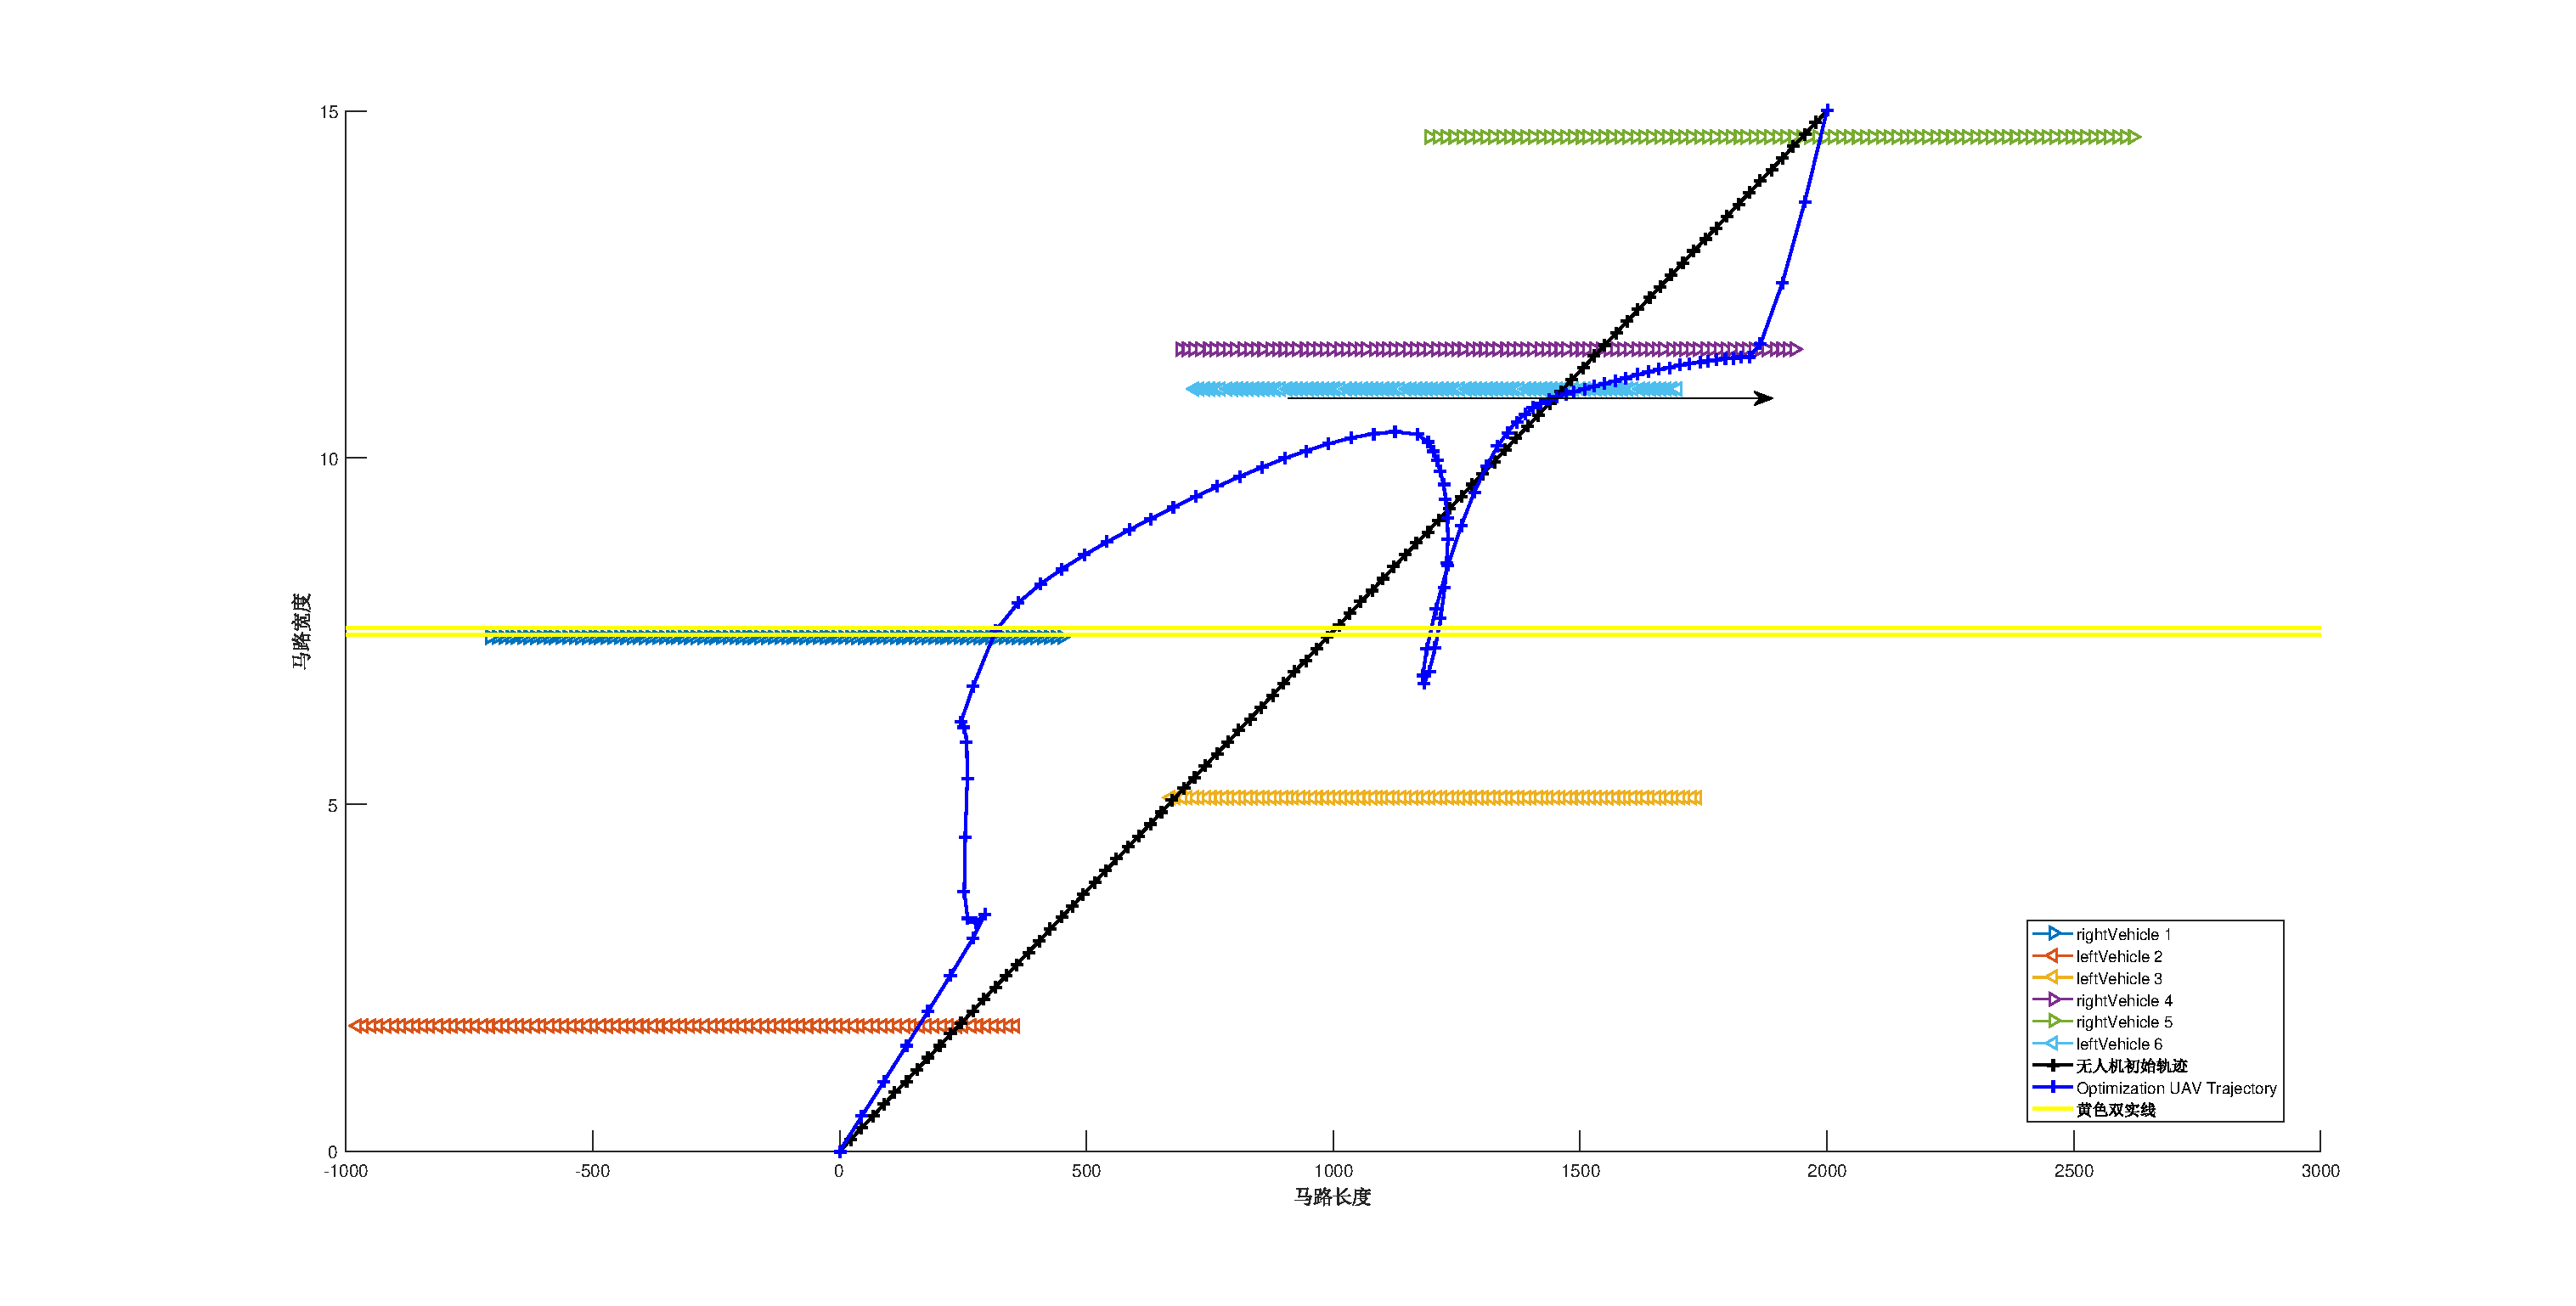
\includegraphics[width=17cm]{figures//chap4//轨迹.eps}
\caption{轨迹.}
\label{F7}
\end{figure}

\begin{figure}[H]
\centering
\includegraphics[width=7cm]{figures//chap4//untitled.eps}
\caption{轨迹.}
\label{F7}
\end{figure}

\section{本章小结}\label{section4-6}

表格的引用同样是使用\verb|\ref{}| 命令实现的。例如“表\verb|\ref{tab:ysubof}|” 输出的结果为:表\ref{biao4-1}。\LaTeX 会自动将其替换为表格的编号。例如:
4
的效果如下:\\
注意!从第二章开始应有``本章小结",主要总结本章所做的主要研究工作,研究成果等内容!!!


燕山大学硕士学位论文参考文献规则的表格如表\ref{biao4-1}所示。
%\section{本章小结}\label{section4-7}
\begin{table}[h] %h表示三线表在当前位置插入
\setlength{\abovecaptionskip}{0.05cm} %设置三线表标题与第一条线间距
\centering\small
\caption{{系统仿真参数}}
%\caption{\textbf{The characteristics of various methods}}
%表头文本加黑,但不加黑Table 1.字样,引入包即可:\usepackage[labelfont=bf]{caption}
%\arrayrulecolor{black} %设置三线表线条颜色:黑色
\begin{tabular*}{\hsize}{@{\extracolsep{\fill}}c c c c} %{\hsize}使三线表自适应宽度,c表示文本居中
  \hline
  参数 & 数值 \\
  \hline
  人机高度  & 100 \\
  1地面基站高度 & 222  \\
  地面基站高度面基站高度面基站高度面基站高度  & 2222  \\
  \hline
\end{tabular*}
\end{table}

\begin{comment}
\begin{table}[h] %h表示三线表在当前位置插入
\setlength{\abovecaptionskip}{0.05cm} %设置三线表标题与第一条线间距
\centering\small
\caption{{系统仿真参数}}
%\caption{\textbf{The characteristics of various methods}}
%表头文本加黑,但不加黑Table 1.字样,引入包即可:\usepackage[labelfont=bf]{caption}
%\arrayrulecolor{black} %设置三线表线条颜色:黑色
\begin{tabular*}{\hsize}{@{\extracolsep{\fill}}c c c c} %{\hsize}使三线表自适应宽度,c表示文本居中
  \hline
  参数 & 数值 \\
  \hline
  人机高度  & 100 \\
  1地面基站高度 & 222  \\
  地面基站高度面基站高度面基站高度面基站高度  & 2222  \\
  \hline
\end{tabular*}
\end{table}
\end{comment}

\begin{comment}
\begin{equation}
\begin{aligned}
\max _{ \boldsymbol{P}, \boldsymbol{Q}} & EE(\boldsymbol{P},\boldsymbol{Q}) \\
\text { s.t. }
& Pr\left\{x_m\left[t\right]SNR_{m,R}\left[t\right]+y_m\left[t\right]SNR_{m,U}\left[t\right]\geq S N R_{th}\right\}\geq1-\varepsilon_1, \forall m,t \\
& q_U^{n\mathrm{\ }+1}-q_U^{n\mathrm{\ }}\le tV_{max}, \forall m \\
& x_m\left[t\right] + y_m\left[t\right]=1, \forall m\\
& 0\le p_m\left[t\right]\le p_{max}, \forall m
\end{aligned}
\end{equation}

\begin{eqnarray}
\begin{aligned}
\max _{ \boldsymbol{P}, \boldsymbol{Q}} & EE(\boldsymbol{P},\boldsymbol{Q}) \label{equ-s1a}\\
\text { s.t. }
& Pr\left\{x_m\left[t\right]SNR_{m,R}\left[t\right]+y_m\left[t\right]SNR_{m,U}\left[t\right]\geq S N R_{th}\right\}\geq1-\varepsilon_1, \forall m,t  \label{equ-s2a}\\
& q_U^{n\mathrm{\ }+1}-q_U^{n\mathrm{\ }}\le tV_{max}, \forall m  \label{equ-s3a}\\
& x_m\left[t\right] + y_m\left[t\right]=1, \forall m \label{equ-s4a}\\
& 0\le p_m\left[t\right]\le p_{max}, \forall m  \label{equ-v1a}
\end{aligned}
\end{eqnarray}

\begin{align}
\max _{ \boldsymbol{P}, \boldsymbol{Q}} & EE(\boldsymbol{P},\boldsymbol{Q}) \label{equ-s1a}\\
\text { s.t. }
& Pr\left\{x_m\left[t\right]SNR_{m,R}\left[t\right]+y_m\left[t\right]SNR_{m,U}\left[t\right]\geq S N R_{th}\right\}\geq1-\varepsilon_1, \forall m,t  \label{equ-s2a}\\
& q_U^{n\mathrm{\ }+1}-q_U^{n\mathrm{\ }}\le tV_{max}, \forall m  \label{equ-s3a}\\
& x_m\left[t\right] + y_m\left[t\right]=1, \forall m \label{equ-s4a}\\
& 0\le p_m\left[t\right]\le p_{max}, \forall m  \label{equ-v1a}
\end{align}

\begin{align}
\max _{ \boldsymbol{P}, \boldsymbol{Q}} & EE(\boldsymbol{P},\boldsymbol{Q}) \label{YY}\\
\text { s.t. }
& Pr\left\{x_m\left[t\right]SNR_{m,R}\left[t\right]+y_m\left[t\right]SNR_{m,U}\left[t\right]\geq S N R_{th}\right\}\geq1-\varepsilon_1, \forall m,t  \label{YYa}\\
& q_U^{n\mathrm{\ }+1}-q_U^{n\mathrm{\ }}\le tV_{max}, \forall m  \label{YYb}\\
& x_m\left[t\right] + y_m\left[t\right]=1, \forall m \label{YYc}\\
& 0\le p_m\left[t\right]\le p_{max}, \forall m  \label{equ-v1a}
\end{align}

\begin{subequations}
\renewcommand{\theequation}
{\theparentequation-\arabic{equation}}
\begin{equation}
A = B
\end{equation}
\begin{equation}
C = D
\end{equation}
\end{subequations}

\end{comment}
